\chapter{Situtation de départ - Software (ESP32)}
\label{sec:CodeESP32}

\section{Introduction}
Le microcontrôleur ESP32 est chargé de gérer la communication avec le DSP ainsi que d'héberger l'interface web. Cette section détaille les différents éléments logiciels qui le composent.

\section{Mise en place}
\label{sec:MiseEnPlaceESP}
\subsection{Configuration de l'Arduino IDE}
Afin de programmer l'ESP-32, l'Arduino IDE a été employer afin de réaliser cela. Pour une utilisation optimum, les réglages suivants doivent être fait.\\

Une librairies à installer est la librairie "FastLED.h" de Daniel Garcia :

\begin{figure}[H]
  \centering
  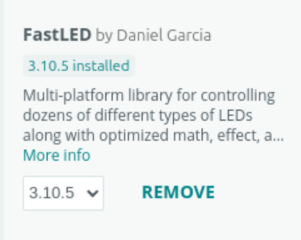
\includegraphics[width=0.5\linewidth]{assets/Chap7/Mise en place/LibInstall.png}
  \caption{Librairie à installer}
  \label{fig:LibInstall}
\end{figure}

Par la suite, le compilateur doit être réglé. Pour commencer, la bonne carte doit être installé. Pour se faire il est néscessaire d'installer dans "Boards Manager" celui d'Espressif Systems concernant l'esp32 :

\begin{figure}[H]
  \centering
  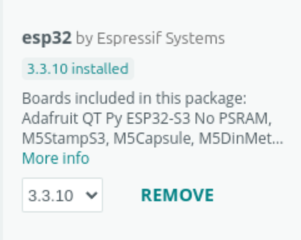
\includegraphics[width=0.5\linewidth]{assets/Chap7/Mise en place/BoardInstall.png}
  \caption{Carte à installer}
  \label{fig:BoardInstall}
\end{figure}

Une fois cela fait, il faut sélectionné la bonne carte. Celle qui nous intéresse est l'ESP32S2 Dev Module :

\begin{figure}[H]
  \centering
  \begin{subfigure}{0.48\textwidth}
    \centering
    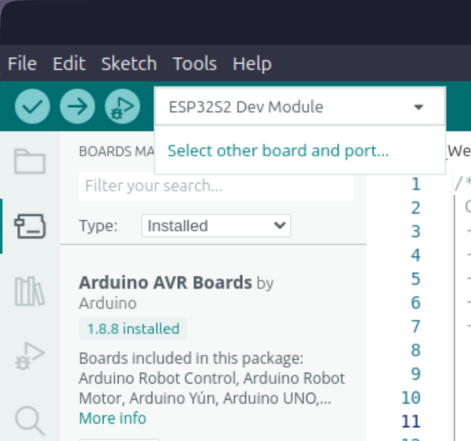
\includegraphics[width=\linewidth]{assets/Chap7/Mise en place/BoardSelect1.png}
    \caption{Première étape}
  \end{subfigure}\hfill
  \begin{subfigure}{0.48\textwidth}
    \centering
    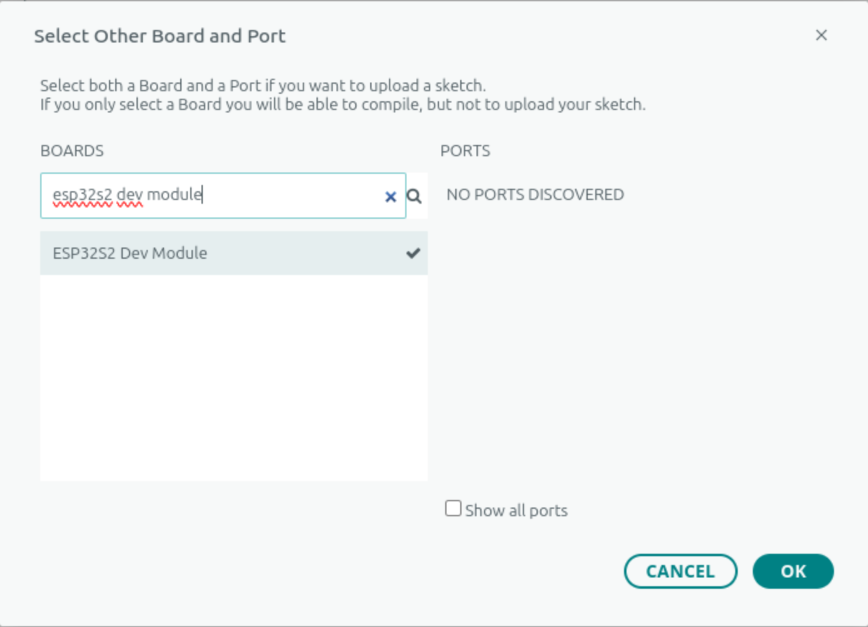
\includegraphics[width=\linewidth]{assets/Chap7/Mise en place/BoardSelect2.png}
    \caption{Deuxième étape}
  \end{subfigure}
  \caption{Étapes à réaliser pour la sélection de la carte}
\end{figure}

Par la suite certaines options doivent être définit dans l'onglet \texttt{Tools} comme démontré dans la \autoref{fig:ToolsSettings}

\begin{figure}[H]
  \centering
  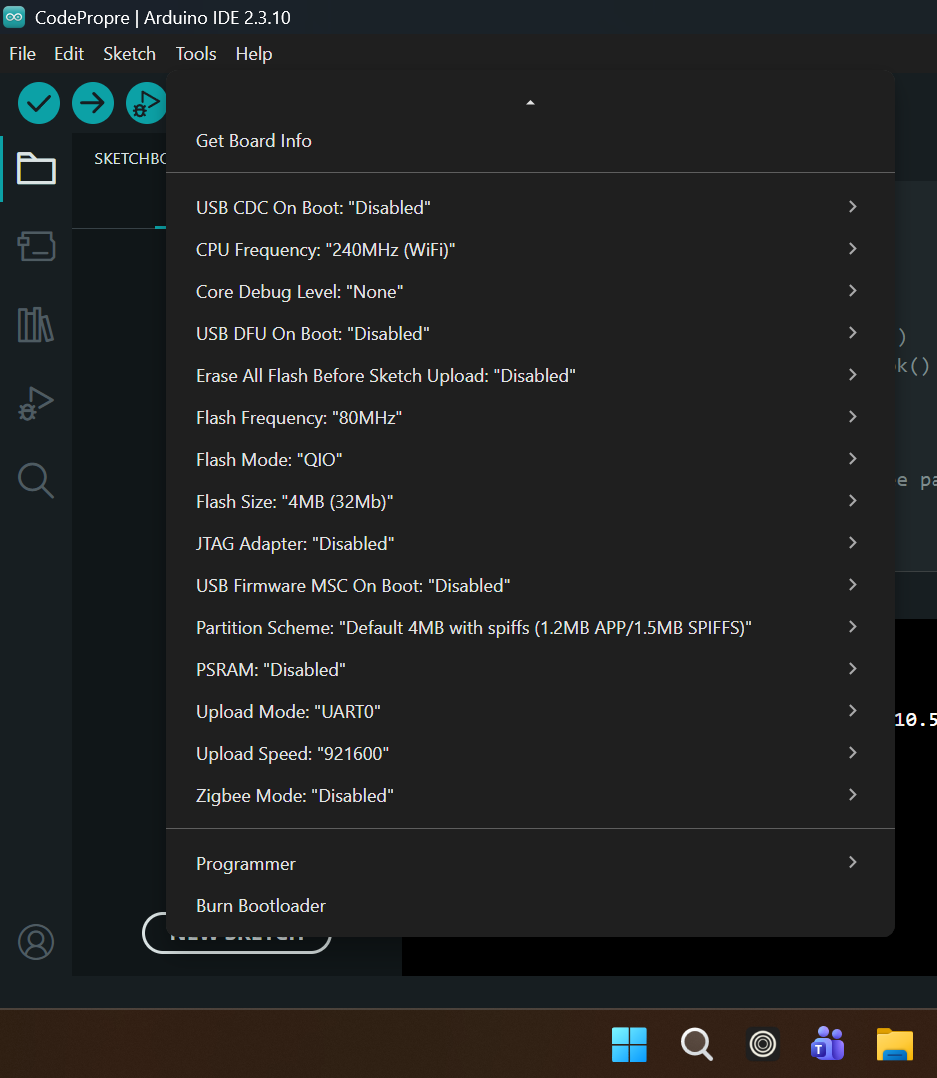
\includegraphics[trim = 0 40 0 0, clip, width=1\linewidth]{assets/Chap7/Mise en place/ToolsSettings.png}
  \caption{Paramètres à définir dans l'onglet \texttt{Tools}}
  \label{fig:ToolsSettings}
\end{figure}

Voici la liste des points à définir :

\begin{enumerate}
  \item USB CDC On Boot Enable
  \item Erase All Flash Before Sketch Upload Enable
  \item cpu speed 240 mhz
  \item flash speed 80 mhz
  \item flash mode qio
  \item flash size 4mb
  \item partition scheme default
\end{enumerate}

Il est dèsormais possible de flasher le code dans l'esp32. Pour se faire, il est néscessaire d'appuyer et maintenir le bouton "Boot" puis pressé une fois sur le bouton "reset". Une fois fait, le code peut-être flasher dans l'esp32. Si une erreur s'affiche dans le terminal de l'arduino, cela est normal et la procédure a tout de même fonctionner

\subsection{Connexion à l'interface web}
Afin de se connecter à l'interface, il est néscessaire de se connecter au WIFI créer par l'ESP-32. Pour cela, les informations suivantes sont néscessaire pour s'y connecter :

\begin{itemize}
  \item Nom du wifi : ESP32-S2-WIFI
  \item Mot de passe : TFE-TB2025-HEIG
  \item Lien du site web : 192.168.4.1
\end{itemize}

Une fois cela réalisé, il est dès alors possible d'intéragir avec le site web.\\

% Actuellement un problème subsiste avec la connexion à la page web. Il arrive qu'au départ le site charge à l'infinie. Pour palier à cela, la méthode trouvé fut de se déconnecter du réseaux de l'esp puis s'y reconnecter après quelque seconde. Ce problème est cependant à régler.

\section{Code Arduino}
Le code Arduino est un programme concis regroupant de nombreuses fonctions dédiées à la communication ainsi qu'à l'affichage de l'interface web.\\

Les bibliothèques employées pour réaliser ces tâches sont les suivantes :

\begin{minted}{c++}
#include <WiFi.h>
#include <WebServer.h>
#include <FastLED.h>
#include <HardwareSerial.h>
#include <stdlib.h>  // Pour atof()
#include <string.h>  // Pour strtok()

#include "WebPage.h"
\end{minted}

Ce programme s'appuie principalement sur les dépendances suivantes :

\begin{itemize}
  \item \texttt{WiFi.h} : Bibliothèque de l'ESP32 permettant la gestion du réseau Wi-Fi. Elle est utilisée pour configurer le microcontrôleur en point d'accès.
  \item \texttt{WebServer.h} : Bibliothèque permettant d'héberger un serveur web et de répondre aux requêtes des utilisateurs.
  \item \texttt{HardwareSerial.h} : Bibliothèque gérant la communication matérielle UART, exploitée pour les échanges de données entre l'ESP32 et le DSP.
  \item \texttt{WebPage.h} : Fichier d'en-tête local contenant le code source de l'interface web (HTML, CSS et JavaScript).
\end{itemize}

Le fonctionnement logiciel est basé sur les travaux de Thomas Freyche et est illustré par l'organigramme de la figure \ref{fig:FoncCodeESP32} :

\begin{figure}[H]
  \centering
  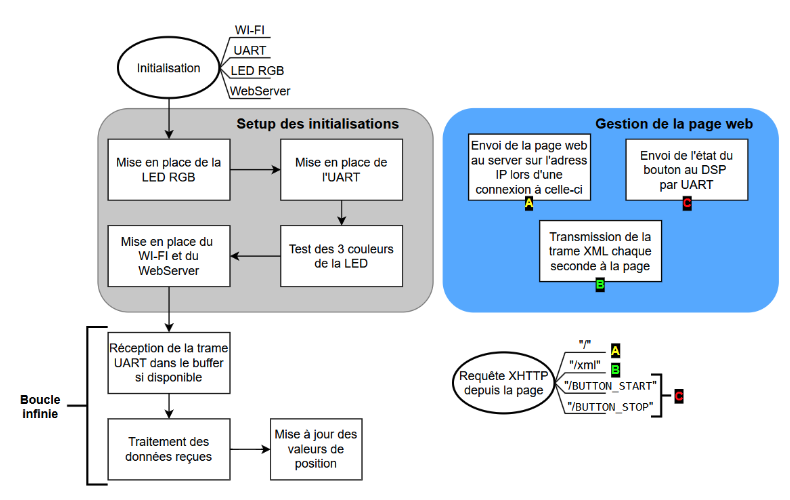
\includegraphics[width=1\linewidth]{assets/Chap7/FonctionnementCode.png}
  \caption{Diagramme du fonctionnement du code de l'ESP32 \cite{Freyche}}
  \label{fig:FoncCodeESP32}
\end{figure}

Le programme assure ainsi les fonctionnalités suivantes :

\begin{itemize}
  \item La réception des données provenant du DSP.
  \item Le traitement et le formatage des informations reçues.
  \item La génération et l'hébergement de l'interface web.
  \item L'actualisation dynamique des valeurs affichées sur le portail web.
  \item La construction d'un graphique représentant l'évolution de la position en fonction du temps.
  \item L'activation et la désactivation à distance de la maquette.
\end{itemize}

À l'avenir, il sera nécessaire d'intégrer l'affichage en temps réel du courant des inducteurs, ainsi qu'une fonctionnalité permettant la modification à la volée des coefficients de régulation.\\

L'interface web se présente telle qu'illustrée sur la figure \ref{fig:Interface} :

\begin{figure}[H]
  \centering
  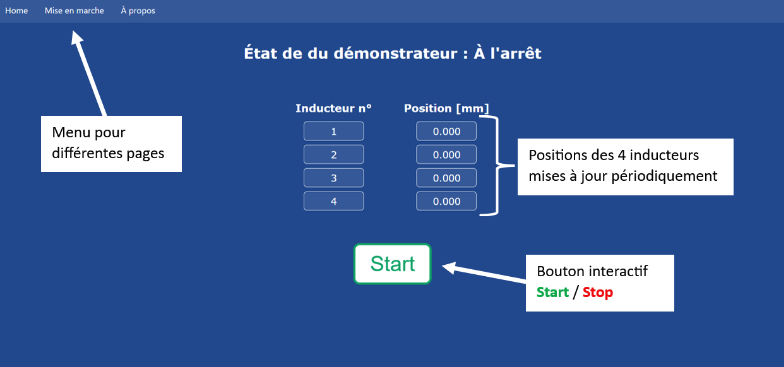
\includegraphics[width=1\linewidth]{assets/Chap7/interface.png}
  \caption{Affichage de l'interface utilisateur - page de lancement à distance \cite{Freyche}}
  \label{fig:Interface}
\end{figure}

La structure de cette interface est définie dans un fichier secondaire intégré au projet. Elle regroupe :

\begin{itemize}
  \item Les langages HTML et CSS définissant l'architecture et l'esthétique de la page.
  \item Le langage JavaScript gérant l'interactivité et la dynamique des éléments (actions sur les boutons, actualisation des métriques, mise à jour du graphique).
\end{itemize}

\section{Analyse de l'espace mémoire}
Le compilateur de l'environnement Arduino permet d'évaluer l'espace mémoire occupé au sein de l'ESP32. L'issue de la compilation fournit les informations suivantes concernant l'allocation mémoire :

\begin{quote}
  Le croquis utilise 979768 octets (74\,\%) de l'espace de stockage de programmes. Le maximum est de 1310720 octets.

  Les variables globales utilisent 45324 octets (13\,\%) de mémoire dynamique, ce qui laisse 282356 octets pour les variables locales. Le maximum est de 327680 octets.
\end{quote}

En ce qui concerne la taille des fichiers sources, le code propre à l'ESP32 représente 9,9~ko, tandis que celui définissant l'interface web occupe 10,6~ko.

\section{Modifications sur la page web et la communication}

\subsection*{Améliorations de l'Interface Web et de la Communication}

\subsubsection*{1. Résolution du problème de chargement infini (Serveur Web)}
Le blocage systématique lors de la connexion initiale à la page web a été résolu par deux interventions logicielles majeures sur l'ESP32 :
\begin{itemize}
  \item \textbf{Correction des codes de statut HTTP :} Les fonctions de réponse du serveur (via la méthode \texttt{server.send()}) renvoyaient initialement le code \texttt{250}. Ce code n'étant pas un standard de succès HTTP, les navigateurs web restaient en attente d'une confirmation. Ce code a été remplacé par le code standard \texttt{200} (OK), validant ainsi immédiatement la complétion de la requête.
  \item \textbf{Désengorgement de la boucle principale (\textit{Main Loop}) :} La lecture ininterrompue du buffer série (\texttt{while (MySerial.available() > 0)}) monopolisait les ressources processeur de l'ESP32 en présence d'un flux de données élevé en provenance du DSP. Une limite logicielle a été introduite (\texttt{bytesToRead = 128}) pour forcer le microcontrôleur à sortir de la boucle de lecture matérielle, libérant ainsi du temps de calcul pour le traitement des requêtes clients WiFi (\texttt{server.handleClient()}).
\end{itemize}

\subsubsection*{2. Intégration de l'affichage des courants}
Afin de superviser simultanément la position et le courant des quatre inducteurs, la chaîne de communication globale a été restructurée pour transmettre 8 variables flottantes (au lieu de 4) :
\begin{itemize}
  \item \textbf{Côté DSP (\texttt{C2000}) :} La taille du buffer d'émission (\texttt{TX\_BUF\_LEN}) a été augmentée de 64 à 128 octets pour éviter les débordements de mémoire. Le prototype et la définition de la fonction \texttt{SendFloatAsText()} ont été modifiés pour accepter 8 arguments, permettant de concaténer et d'envoyer la trame complète en une seule interruption série.
  \item \textbf{Côté Microcontrôleur WiFi (\texttt{ESP32-S2}) :} Le buffer de réception (\texttt{UART\_BUFFER}) a été proportionnellement agrandi. La fonction de \textit{parsing} (découpage de la trame via \texttt{strtok}) a été ajustée pour extraire itérativement jusqu'à 8 valeurs. Ces données sont ensuite formatées dans le serveur web en injectant de nouvelles balises XML dédiées (\texttt{<curIndX>}).
  \item \textbf{Côté Client Web (\texttt{HTML/JS}) :} L'interface a été enrichie d'une nouvelle structure en colonne (DOM). Le script JavaScript asynchrone gérant la communication AJAX a été complété pour extraire les données de courant du flux XML, traiter la conversion des virgules en points, et actualiser dynamiquement l'affichage en temps réel.
\end{itemize}

\subsubsection*{3. Optimisation pour l'affichage mobile (\textit{Responsive Design})}
Pour pallier le chevauchement et le débordement des éléments graphiques sur des écrans étroits (smartphones), le code CSS de l'interface a été remanié :
\begin{itemize}
  \item \textbf{Restructuration de la mise en page :} Implémentation d'une disposition en boîte flexible (\texttt{flex-wrap: wrap}) sur le conteneur principal pour autoriser le retour à la ligne des éléments si nécessaire.
  \item \textbf{Requêtes multimédias (\textit{Media Queries}) :} Ajout d'une règle d'adaptation conditionnelle (\texttt{@media (max-width: 600px)}). Cette règle réduit dynamiquement l'espacement inter-colonnes (\texttt{gap}), les marges internes (\texttt{padding}), la taille des polices d'écriture (\texttt{font-size}) et la largeur absolue des cellules d'affichage lorsque la résolution horizontale de l'écran est critique.
\end{itemize}

\subsubsection*{4. Déploiement d'un graphique dynamique (Oscilloscope virtuel)}
Afin de faciliter l'analyse du comportement transitoire du système de sustentation, un outil de visualisation temporelle a été ajouté à la page web :
\begin{itemize}
  \item \textbf{Technologie autonome :} L'ESP32 générant un réseau local sans accès à Internet, l'utilisation de bibliothèques tierces (comme \textit{Chart.js}) était impossible. Le graphique a été entièrement implémenté en utilisant l'élément natif HTML5 \texttt{<canvas>} et un script JavaScript dédié.
  \item \textbf{Fenêtre glissante et chronométrie :} L'axe temporel (abscisse) utilise l'horloge interne du navigateur (\texttt{Date.now()}) pour garantir un défilement rigoureusement fluide. La zone d'affichage agit comme une fenêtre glissante de 10 secondes synchronisée au clic sur le bouton de démarrage, simulant avec précision le comportement d'un oscilloscope classique.
\end{itemize}

\subsubsection*{5. Débogage et validation physique de la machine d'états}
Lors des essais d'intégration, une anomalie a été identifiée grâce à la télémétrie web : bien que la position réponde correctement, le courant restait figé autour de 3A (valeur de pré-décollage), et ce même lorsque l'inducteur entrait en contact physique avec l'aimant.
\begin{itemize}
  \item \textbf{Déduction théorique :} Selon la loi de commande implémentée ($i_c = \sqrt{K_{FC} \cdot f_c} \cdot z$), si l'entrefer $z$ devient nul (inducteur collé), le courant de consigne $i_c$ devrait théoriquement s'annuler de manière instantanée.
  \item \textbf{Correction logicielle :} L'analyse du flux d'exécution a révélé que le DSP restait bloqué indéfiniment dans l'état de préparation au décollage (\texttt{STATE\_1}). La condition de transition exigeait la stabilisation stricte de deux inducteurs simultanément. En isolant la condition pour réaliser les tests sur un seul inducteur, la machine d'états a pu basculer en mode de régulation nominale (\texttt{STATE\_3}), confirmant la justesse de l'hypothèse physique et le bon fonctionnement de l'asservissement en espace d'état.
\end{itemize}

\section{A faire}
\begin{itemize}
  \item Ajouter la mesure de courant
  \item Régler le chargement infinie de la page
  \item Créer un QR code pour se connecter à la page
  \item Ajouter un slider pour changer les coeffs des réguls
\end{itemize}
